\section[The Riemann-Stieltjes Integral]{\hyperlink{toc}{The Riemann-Stieltjes Integral}}

\subsection{Definition of the Integral}
\begin{definition}{Partition}{6.1}
    A \textbf{partition} of $[a, b] \subset \RR$ is a set $\set{x_0, x_1, \ldots, x_n}$ (for some $n \in \NN$) such that:
    \begin{align*}
        a = x_0 \leq x_1 \leq x_2 \leq \ldots \leq x_{n-1} \leq x_n = b
    \end{align*}
    We can then write:
    \begin{align*}
        \Delta x_i = x_i - x_{i-1} 
    \end{align*}
\end{definition}

\begin{figure}[htbp]
    \centering
    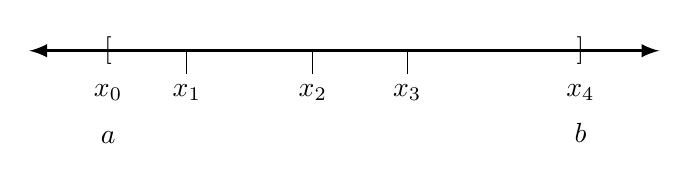
\begin{tikzpicture}[scale=2]
        \draw[very thick, latex-latex] (-2, 0) -- (2, 0);
        \node[] at (-1.5, 0) {$[$};
        \node[below] at (-1.5, -0.15) {$x_0$};
        \node[below] at (-1.5, -0.45) {$a$};
        \node[] at (1.5, 0) {$]$};
        \node[below] at (1.5, -0.15) {$x_4$};
        \node[below] at (1.5, -0.4) {$b$};
        \draw[] (-1, 0) -- (-1, -0.15);
        \node[below] at (-1, -0.15) {$x_1$};
        \draw[] (-0.2, 0) -- (-0.2, -0.15);
        \node[below] at (-0.2, -0.15) {$x_2$};
        \draw[] (0.4, 0) -- (0.4, -0.15);
        \node[below] at (0.4, -0.15) {$x_3$};
    \end{tikzpicture}
    \caption{Visualization of a partition $\set{x_0, x_1, x_2, x_3, x_4}$ of $[a, b]$. Note that the points in the partitions need not be equally spaced.}
    \label{fig27}
\end{figure}

\setcounter{rudin}{0}
\begin{definition}{Upper and Lower Sums}{6.1}
    Given $f: [a, b] \mapsto \RR$ and a partition $P$ of $[a, b]$ let:
    \begin{align*}
        M_i &= \sup\set{f(x): x_{i-1} \leq x \leq x_i}
        \\ m_i &= \inf\set{f(x): x_{i-1} \leq x \leq x_i}
    \end{align*}
    Then, we can define the \textbf{upper} and \textbf{lower sums}:
    \begin{align*}
        U(P, f) &= \sum_{i=1}^n M_i \Delta x_i
        \\ L(P, f) &= \sum_{i=1}^n m_i \Delta x_i
    \end{align*}
\end{definition}

\begin{figure}[htbp]
    \centering
    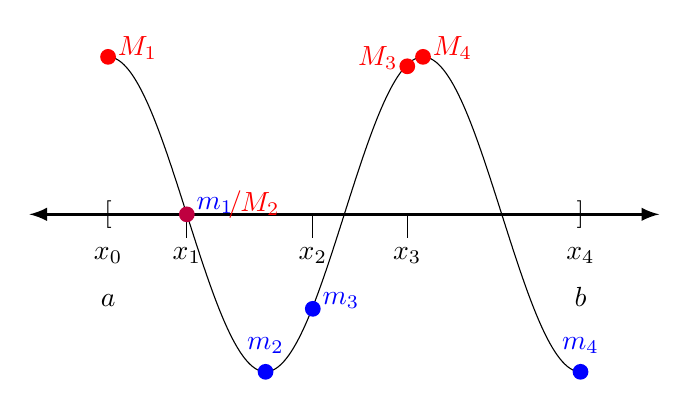
\begin{tikzpicture}[scale=2]
        \draw[very thick, latex-latex] (-2, 0) -- (2, 0);
        \node[] at (-1.5, 0) {$[$};
        \node[below] at (-1.5, -0.15) {$x_0$};
        \node[below] at (-1.5, -0.45) {$a$};
        \node[] at (1.5, 0) {$]$};
        \node[below] at (1.5, -0.15) {$x_4$};
        \node[below] at (1.5, -0.4) {$b$};
        \draw[] (-1, 0) -- (-1, -0.15);
        \node[below] at (-1, -0.15) {$x_1$};
        \draw[] (-0.2, 0) -- (-0.2, -0.15);
        \node[below] at (-0.2, -0.15) {$x_2$};
        \draw[] (0.4, 0) -- (0.4, -0.15);
        \node[below] at (0.4, -0.15) {$x_3$};
        \draw[] (-1, 0) sin (-1.5, 1);
        \draw[] (-1, 0) sin (-0.5, -1);
        \draw[] (0, 0) sin (-0.5, -1);
        \draw[] (0, 0) sin (0.5, 1);
        \draw[] (1, 0) sin (0.5, 1);
        \draw[] (1, 0) sin (1.5, -1);
        \node[circle, fill = red, minimum size = 0.2cm, inner sep = 0pt, label={[right, text=red]:$M_1$}] at (-1.5, 1) {};
        \node[circle, fill = purple, minimum size = 0.2cm, inner sep = 0pt, label={[right, text=blue]:$m_1$}] at (-1, 0) {};
        \node[right, text = red] at (-0.8, 0.06) {$/M_2$};
        \node[circle, fill = blue, minimum size = 0.2cm, inner sep = 0pt, label={[above, text=blue]:$m_2$}] at (-0.5, -1) {};
        \node[circle, fill = blue, minimum size = 0.2cm, inner sep = 0pt, label={[right, text=blue]:$m_3$}] at (-0.2, -0.6) {};
        \node[circle, fill = red, minimum size = 0.2cm, inner sep = 0pt, label={[left, text=red]:$M_3$}] at (0.4, 0.94) {};
        \node[circle, fill = red, minimum size = 0.2cm, inner sep = 0pt, label={[right, text=red]:$M_4$}] at (0.5, 1) {};
        \node[circle, fill = blue, minimum size = 0.2cm, inner sep = 0pt, label={[above, text=blue]:$m_4$}] at (1.5, -1) {};
        \end{tikzpicture}
    \caption{Example of a function $f$, a partition $P$ of $[a, b]$, and the $M_i, m_i$s for this choice of partition.}
    \label{fig28}
\end{figure}

\noindent By construction, it should be evident that $L(P, f) \leq U(P, f)$ for all $P, f$.

A natural question that arises from the form of the above expression is whether these are Riemann sums or not. Recall from first year calculus that we would choose the left endpoint, right endpoint, or some other arbitrary choice of a point in the subinterval. Here, we in a sense use a ``special case'' of the supremum/infimum. We will see that this choice is musch easier to use in proofs due to monotonicity properties. Namely, if we have a partition and add another point, then $U(P, f)$ can only decrease, and $L(P, f)$ can only increase (we will see this in a theorem soon)!


\setcounter{rudin}{0}
\begin{definition}{Upper/Lower Integrals and Riemann Integrability}{6.1}
    We define the \textbf{upper Riemann integral} to be:
    \begin{align*}
        \uint{a}{b} = \inf_P U(P, f).
    \end{align*}
    and the \textbf{lower Riemann integral} to be:
    \begin{align*}
        \lint{a}{b} = \sup_P L(P, f).
    \end{align*}
    Here, the infimum/supremum is taken over all partitions $P$. We say that $f$ is \textbf{Riemann integrable} on $[a, b]$, and write $f \in \R[a, b]$ if:
    \begin{align*}
        \uint{a}{b} = \lint{a}{b}
    \end{align*}
    which we can write as:
    \begin{align*}
        \int_{a}^{b} f dx \text{ or } \int_{a}^{b} f(x) dx
    \end{align*}
\end{definition}
\noindent Note that the choice of variable in the above definition is totally arbitrary. 

Also, note that while $f$ is not required to be continuous in the above definition, it is required to be bounded; else, $M_i$ and $m_i$ may not exist. Since $f$ is bounded, $U(P, f)$, $L(P, f)$ are bounded for all $P, f$ and hence we have a set of real numbers for which we may consider the supremum/infimium of by the LUB/GLB property of the reals. Since the upper/lower sums lie in a bounded interval, there is no questions about whether the lower/upper integrals exist. The question becomes whether they are equal or not. Before getting into further discussion on this topic, we discuss a bound:

\setcounter{rudin}{0}
\begin{theorem}{ML Bounds}{6.1}
    Let $m = \inf\set{f(x): a \leq x \leq b}$ and $M = \sup\set{f(x): a \leq x \leq b}$ (which exist by the boundedness of $f$). Then,
    \begin{align*}
        m(b - a) \leq L(P, f) \leq U(P, f) \leq M(b - a)
    \end{align*}
    For any choice of partition $P$.
\end{theorem}
\begin{nproof}
    For any $i$, we have that:
    \begin{align*}
        m \leq m_i \leq M_i \leq M
    \end{align*}
    Therefore:
    \begin{align*}
        \sum_{i=1}^n m \Delta x_i \leq \sum_{i=1}^n m_i \Delta x_i \leq \sum_{i=1}^n M_i \Delta x_i \leq \sum_{i=1}^n M \Delta x_i
    \end{align*}
    So we conclude that:
    \begin{align*}
        m(b - a) \leq L(P, f) \leq U(P, f) \leq M(b - a)
    \end{align*} \qed
\end{nproof}

\noindent Now that we have established the Riemann integral, a natural question is how can we extend this notion. In order to do so, we will use a montonically increasing function $\alpha: [a, b] \mapsto \RR$ (that is, $\alpha(x) \leq \alpha(y)$ for all $x \leq y$). Note that $\alpha$ need not be continuous. Indeed, compared to the Riemann integral where $\alpha(x) = x$ and was continuous, in this general setting, $\alpha$ is allowed to have jumps. This allows for certain benefits, as we will soon discuss. However, we note that $\alpha$ can only have a finite number of jumps.

\begin{ntheorem}{ 4.30}{}
    Let $\alpha: [a, b] \mapsto \RR$ be monotonic. Then, it can only have finitely many discontinities.
\end{ntheorem}
\begin{nproof}
    Assign a rational number $r(x)$ to each of the discontinuities of $\alpha$. Then, we have that:
    \begin{align*}
        \lim_{x \rightarrow r(x)^-} \alpha(x) < \alpha(x) < \lim_{x \rightarrow r(x)^+} \alpha(x)
    \end{align*}
    Since $x_1 < x_2$ implies $\lim_{x \rightarrow r(x_1)^+} \alpha(x) \leq lim_{x \rightarrow r(x_2)^-} \alpha(x)$, we have that $r(x_1) \neq r(x_2)$ if $x_1 \neq x_2$. We therefore have established a function $r$ from the set of discontinuities of $\alpha$ to the rationals. As the rationals are countable, the set of discontiuities of $\alpha$ are also countable. \qed
\end{nproof}

\noindent With this established, we now define the generalized Riemann-Stieltjes integral.

\begin{definition}{Riemann-Stieltjes Integral}{6.2}
    Let $\alpha: [a, b] \mapsto \RR$ be increasing, and given a partition $P$ of $[a, b]$, define:
    \begin{align*}
        \Delta \alpha_i = \alpha(x_i) - \alpha(x_{i-1}) (\geq 0)
    \end{align*}
    For bounded $f: [a, b] \mapsto \RR$, Let:
    \begin{align*}
        U(P, f, \alpha) &= \sum_{i=1}^n M_i \Delta \alpha_i
        \\ L(P, f, \alpha) &= \sum_{i=1}^n m_i \Delta \alpha_i
    \end{align*}
    We then take the infimum/supremum over partitions $P$ to get:
    \begin{align*}
        \uint{a}{b} f d\alpha &= \inf_P U(P, f, \alpha)
        \\ \lint{a}{b} &= \sup_P L(P, f, \alpha)
    \end{align*}
    If equal, we write their value as:
    \begin{align*}
        \int_a^b f d\alpha \text{ or } \int_a^b f(x)d\alpha(x)
    \end{align*}
    and we write that $f \in \R_\alpha[a, b]$. In the case where $\alpha(x) = x$, we recover the Riemann integral.
\end{definition}

\noindent Why is this definition useful? What does it accomplish for us that the original Riemann integral does not? We consider a physically motivating example. Suppose we have a thin wire with varying mass density $\rho(x)$. If we wanted to calculate the mass density of the wire, we would integrat the density $\rho(x)$ over the length of the wire. Now, suppose our wire consists of steel of continuously varying mass density, as well as beads/point masses placed on certain locations of the wire. The Riemann integral cannot handle these point masses, but the Riemann-Stieltjes integral can deal with this case if we use an $\alpha$ with discontinuities in it. Hence, the Riemann-Stieltjes integral allows us to handle cases where we both have continuous and discrete masses to integrate over. It acts as a bridge between Riemann and Lebesgue integration (the latter of which will be the subject of a later course in measure theory).

We now will answer the question: ``for what choices of $f, \alpha$ is $f$ Riemann-Stieltjes integrable?''

\subsection{Criterion for Integrability}

\begin{definition}{Refinements and Common Refinemnet}{6.3}
    $P^*$ is a \textbf{refinement} of $P$ if $P \subset P^*$ and $P, P^*$ are partitions. The common refinemnet of $P_1, P_2$ is $P^* = P_1 \cup P_2$.
\end{definition}

\begin{theorem}{}{6.4}
    If $P^*$ is a refinemne tof $P$, then:
    \begin{align*}
        L(P, f, \alpha) \leq L(P^*, f, \alpha) \leq U(P^*, f, \alpha) \leq U(P, f, \alpha)
    \end{align*}
\end{theorem}

\noindent As a remark, when we take infimums/supremums over partitions $P$ to obtain the upper/lower Riemann-Stieltjes integals, we are taking refinements.

Also, note that the above theorem does \textit{not} apply to (right-hand, left-hand, midpoint, arbitrary) Riemann sums, and is a consequence of the choice of upper/lower sums with supremums/infimums taken over the subintervals.




\subsection{Properties of the Integral}

\subsection{Integration and Differentiation}

